% Parte II: Integração numérica
% - Integração numérica: ideia básica, métodos básicos (Euler explícito e implícito, RKs); comentar um pouco sobre os outros métodos do tipo que existem.
% - Métodos simpléticos:
%   - Panorama geral; existência de hamiltoniana perturbada (backward error analysis)
%   - Ideia básica para hamiltonianas separáveis; construção de métodos via exponenciais; Métodos básicos: Euler semi-implícito, Velocity-Verlet, Ruth 3 e 4;
%   - O que fazer com hamiltonianas não separáveis?
%   - Métodos de Runge-Kutta-Nystrom (ordens 5 e 6), ou Partitioned Runge-Kutta methods;
%   - Métodos de alta ordem via composição de métodos de baixa ordem: Stormer-Verlet Composto 8 e 10.
% - O que mais é possível no mundo de integradores?
%   - Métodos de passo múltiplo.
%   - Timestep variável, casos tradicional e simplético.
%   - Block-timesteps para problemas multiescala. Versão tradicional e versão simplética. Questões.
% - Correção numérica baseada em integrais primeiras. Ideia, vantagens e desvantagens.
%
\begin{frame}[plain]
    \centering
    \vspace{0.5cm}
    \Huge Parte III: Integração numérica
    
    \vspace{0.7cm}
    \large
    \begin{itemize}
        \item Métodos de passo único;
        \item Métodos simpléticos;
        \item Corretor numérico;
        \item Métodos multipasso.
    \end{itemize}
\end{frame}

%------------------------------------------------

\begin{frame}
\justifying
\frametitle{Métodos de passo único (1/2)}
    Servem para quaisquer PVI de EDO bem-posto:
    $$
    \vet y'(t) = \vet f(t, \vet y(t)), \quad \vet y(t_0) = \vet y_0.
    $$
    São obtidos pensando-se na série de Taylor da solução.

    \begin{columns}[c]
        \column{.65\textwidth}\justifying
            \begin{block}{Métodos de passo único}
                $$
                \vet y(t_k + h) \approx \vet y_{k+1} = \vet y_k + h \vet \Phi_h(\vet y_k, \vet y_{k+1}).
                $$
            \end{block}
            \pause
            \begin{exampleblock}{Exemplos de 1ª ordem}
                \begin{itemize}
                    \item Euler Explícito: $\vet y_{k+1} = \vet y_k + h \vet f(t_k, \vet y_k)$.
                    \item Euler Implícito: $\vet y_{k+1} = \vet y_k + h \vet f(t_{k+1}, \vet y_{k+1})$.
                \end{itemize}
            \end{exampleblock}
        
        \column{.35\textwidth}\justifying
            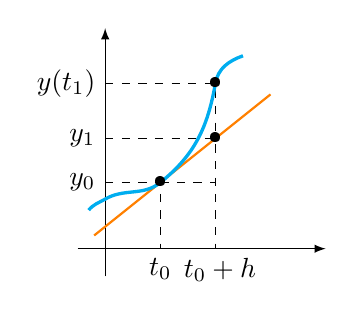
\begin{tikzpicture}[x=0.7cm,y=0.7cm]\centering
                \draw[-latex] (-0.5,0)--(4,0); % eixo x
                \draw[-latex] (0,-0.5)--(0,4); % eixo y

                \draw[dashed] (0,1.2) node[left] {$y_0$}--(1,1.2)--(1,0) node[below] {$t_0$}; % y0 -- * -- t0
                \draw[dashed] (1,1.2)--(2,1.2)--(2,0) node[below] {$\ t_0+h$}; % * -- * -- t_1 = t0+h
                \draw[dashed] (0,2) node[left] {$y_1$}--(2,2)--(2,1.2); % y1 -- * -- t_1 = t0+h
                \draw[dashed] (0,3) node[left] {$y(t_1)$}--(2,3)--(2,2); % y(t1) -- * -- *

                % reta passando pelos pontos (t0, y0) e (t0+h,y1)
                \draw[thick, orange] (-0.2,0.24) -- (3,2.8);

                % a curva
                \draw[very thick, cyan] (-0.3,0.7) 
                to[out=50,in=210] (0,0.9) 
                to[out=30,in=218.66] (1,1.2) 
                to[out=38.66,in=260] (2,3)
                to[out=80,in=200] (2.5,3.5);

                % pontos pretos (bullet)
                \foreach \Point in {(1,1.2),(2,2),(2,3)}{
                    \node at \Point {\textbullet};
                }
            \end{tikzpicture}
    \end{columns}
    \vspace{0.5cm}
    \pause
    \begin{itemize}
        \item Podemos usar várias $f$ fazendo uma média ponderada. Esses são os métodos de Runge-Kutta!
    \end{itemize}
\end{frame}

%------------------------------------------------

% \begin{frame}
% \justifying
% \frametitle{Métodos de Runge-Kutta (2/3)}
%     Podemos usar uma média ponderada de $f$ para aproximar melhor a série. Esses são os Runge-Kutta!

%     \begin{exampleblock}{Exemplo de Runge-Kutta de ordem 4 e 4 estágios (RK44)}
%         $$
%         \vet y_{k+1} = \vet y_k + \dfrac{h}{6} (\vet \kappa_1 + 2 \vet \kappa_2 + 2 \vet \kappa_3 + \vet \kappa_4),
%         $$
%         onde:
%         \begin{align*}
%             \vet \kappa_1 &= f\left(t_k, \vet y_k \right), \\
%             \vet \kappa_2 &= f\left(t_k + \dfrac{h}{2}, \vet y_k + \dfrac{h}{2} \vet \kappa_1 \right), \\
%             \vet \kappa_3 &= f\left(t_k + \dfrac{h}{2}, \vet y_k + \dfrac{h}{2} \vet \kappa_2 \right), \\
%             \vet \kappa_4 &= f\left(t_k + h, \vet y_k + h \vet \kappa_3 \right).
%         \end{align*}
%     \end{exampleblock}

% \end{frame}

%------------------------------------------------

\begin{frame}
\justifying
\frametitle{Testes com métodos de passo único gerais (2/2)}
    \begin{columns}[c]
    \column{.50\textwidth}\justifying
        \begin{figure}
            \centering
            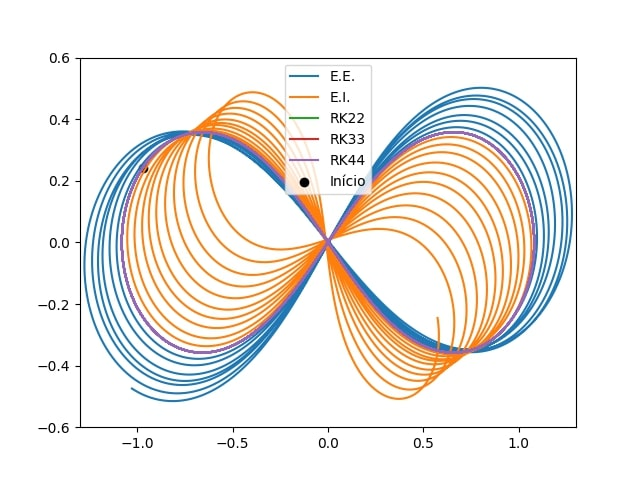
\includegraphics[width=\linewidth]{img/trajetorias_tradicionais.jpg}
            \caption{Lemniscata com $h=10^{-3}$}
        \end{figure}
    
    \column{.50\textwidth}\justifying
        \begin{figure}
            \centering
            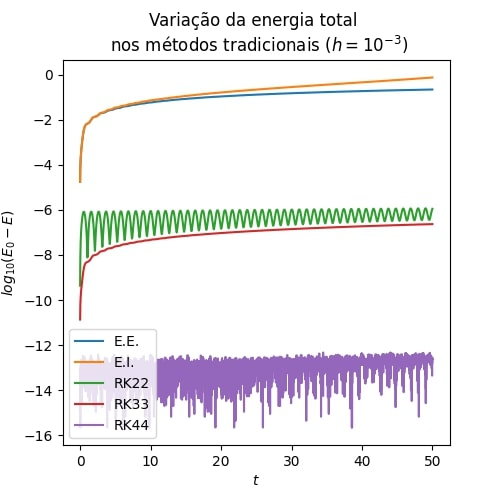
\includegraphics[width=\linewidth]{img/var_energia_tradicionais.jpg}
            \caption{Variação da energia total na lemniscata com $h=10^{-3}$.}
        \end{figure}
    \end{columns}
\end{frame}

%------------------------------------------------
%------------------------------------------------
%------------------------------------------------

\begin{frame}
\justifying
\frametitle{Integração numérica: Métodos simpléticos (1/13)}

\begin{columns}[c]
    \column{.50\textwidth}\justifying
        \begin{block}{Métodos gerais}
            \begin{itemize}
                \item Consideram:
                    \begin{itemize}
                        \item Valor inicial;
                        \item Derivada.
                    \end{itemize}

                \pause

                \item $\Rightarrow$ Equação modificada tem geometria própria.

                \pause

                \item $\Rightarrow$ Erro na energia: $c \cdot t^{1/2}$ \cite{Brouwer1937}

                \pause
            \end{itemize}
        \end{block}
        
    \column{.50\textwidth}\justifying
        \begin{block}{Métodos simpléticos}
            \begin{itemize}
                \item Consideram:
                    \begin{itemize}
                        \item Valor inicial;
                        \item Derivada;
                        \item Geometria do sistema!
                    \end{itemize}

                \pause

                \item $\Rightarrow$ Equação modificada tem a mesma geometria!

                \pause

                \item $\Rightarrow$ Hamiltoniana modificada.
            \end{itemize}
        \end{block}
\end{columns}

\pause

\begin{block}{Caracterização}
    A aplicação $\Psi_k: \vet z_k \to \vet z_{k+1}$, $\vet z_k = (\vet q_k, \vet p_k)$, é simplética se:
    \begin{equation}
        (D \Psi_h) \bm \Omega (D \Psi_h)^T = \bm \Omega.
    \end{equation}
\end{block}

\begin{exampleblock}{}
    Aplicações simpléticas preservam área.
\end{exampleblock}

\end{frame}

%------------------------------------------------

\begin{frame}
\justifying
\frametitle{Construção de métodos para hamiltonianas separáveis (2/13)}

Para uma hamiltoniana separável $H(\vet q, \vet p) = T(\vet p) + V(\vet q)$, separamos o problema em dois:
$$
\begin{cases}
    \dvet q = \nabla_{\vet p} T(\vet p), \\
    \dvet p = \vet 0,
\end{cases}
\quad , \quad
\begin{cases}
    \dvet q = \vet 0, \\
    \dvet p = - \nabla_{\vet q} V(\vet q).
\end{cases}
$$
\pause
Podemos obter os respectivos fluxos explicitamente:
$$
\vet \Phi_{\tau, T}(\vet z) = \begin{bmatrix}
\vet q + \tau \nabla_{\vet p} T(\vet p) \\
\vet p
\end{bmatrix},
\quad
\vet \Phi_{\tau, V}(\vet z) = \begin{bmatrix}
\vet q \\
\vet p - \tau \nabla_{\vet q} V(\vet q)
\end{bmatrix}.
$$
\pause
A aplicação composta $\vet \Phi_\tau = \vet \Phi_{\tau, T} \circ \vet \Phi_{\tau, V}$ é o chamado Método de Euler Simplético (ou semi-implícito):
$$
\vet q_{k+1} = \vet q_k + h \nabla_{\vet p} T(\vet p_k),
\quad
\vet p_{k+1} = \vet p_k - h \nabla_{\vet q} V(\vet q_{k+1}).
$$

\end{frame}

%------------------------------------------------


\begin{frame}
\justifying
\frametitle{Euler explícito vs implícito vs simplético (3/13)}

\begin{columns}[c]
\column{.50\textwidth}\justifying
    \begin{figure}
        \centering
        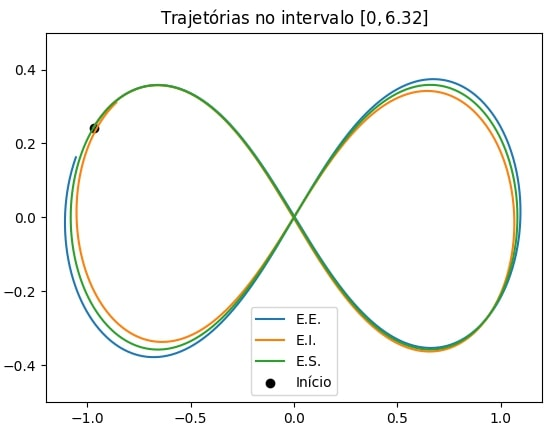
\includegraphics[width=\linewidth]{img/trajetorias_euler.jpg}
    \end{figure}
    
\column{.50\textwidth}\justifying
    \begin{figure}
        \centering
        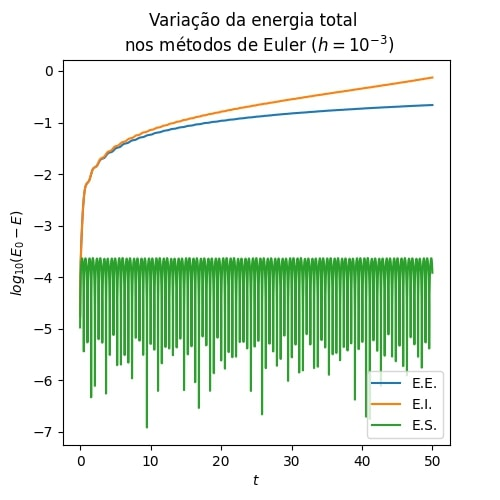
\includegraphics[width=\linewidth]{img/var_energia_euler.jpg}
    \end{figure}
    
\end{columns}

\end{frame}

%------------------------------------------------

\begin{frame}
\justifying
\frametitle{Euler simplético vs Runge-Kuttas (4/13)}

\begin{figure}
    \centering
    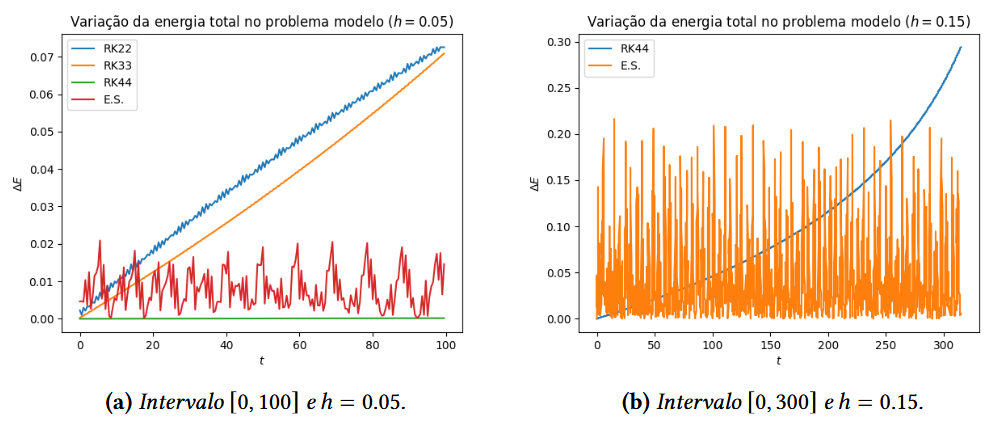
\includegraphics[width=\linewidth]{img/simpleticos_vantagem.png}
    \caption{Variação da energia total na simulação da lemniscata com RK22, RK33, RK44 e Euler Simplético.}
\end{figure}

\end{frame}

%------------------------------------------------

\begin{frame}
\justifying
\frametitle{Euler explícito vs implícito vs simplético (5/13)}

\begin{figure}
    \centering
    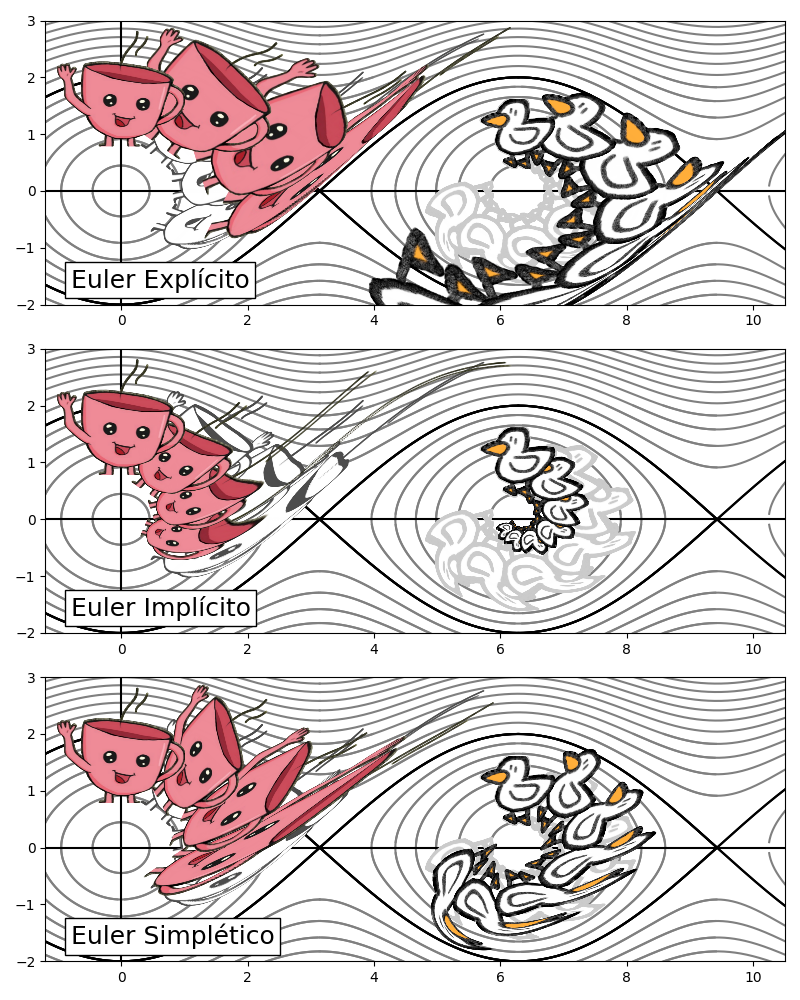
\includegraphics[width=0.47\linewidth]{python/pendulo/eulers.png}
    \caption{Métodos de Euler aplicados no pêndulo com $dt = \pi/4$.}
\end{figure}

\end{frame}

%------------------------------------------------

\begin{frame}
\justifying
\frametitle{Métodos via composição (6/13)}

\begin{itemize}

\item Podemos obter outros métodos simpléticos com mais composições:
$$
\vet \Phi_h = \vet \Phi_{d_s h, V} \circ \vet \Phi_{c_s h, T} \circ \hdots \circ \vet \Phi_{d_1 h, V} \circ \vet \Phi_{c_1 h, T}.
$$

\end{itemize}

\pause

\begin{exampleblock}{Velocity-Verlet}
    Com $d_1 = d_2 = 1/2$ e $c_1 = 0$ e $c_2 = 1$, temos um método consistente, simétrico, explícito, simplético e de 2ª ordem:
    \begin{align*}
        \vet p_{k+1/2} &= \vet p_k - \dfrac{h}{2} \nabla_{\vet q}V(\vet q_k) \\
        \vet q_{k+1} &= \vet q_k + h \nabla_{\vet p} T(\vet p_{k+1/2}), \\
        \vet p_{k+1} &= \vet p_{k+1/2} - \dfrac{h}{2} \nabla_{\vet q}V(\vet q_{k+1})
    \end{align*}
\end{exampleblock}

\end{frame}

%------------------------------------------------

\begin{frame}
\justifying
\frametitle{Runge-Kutta de ordem 2 vs Velocity-Verlet (7/13)}

\begin{figure}
    \centering
    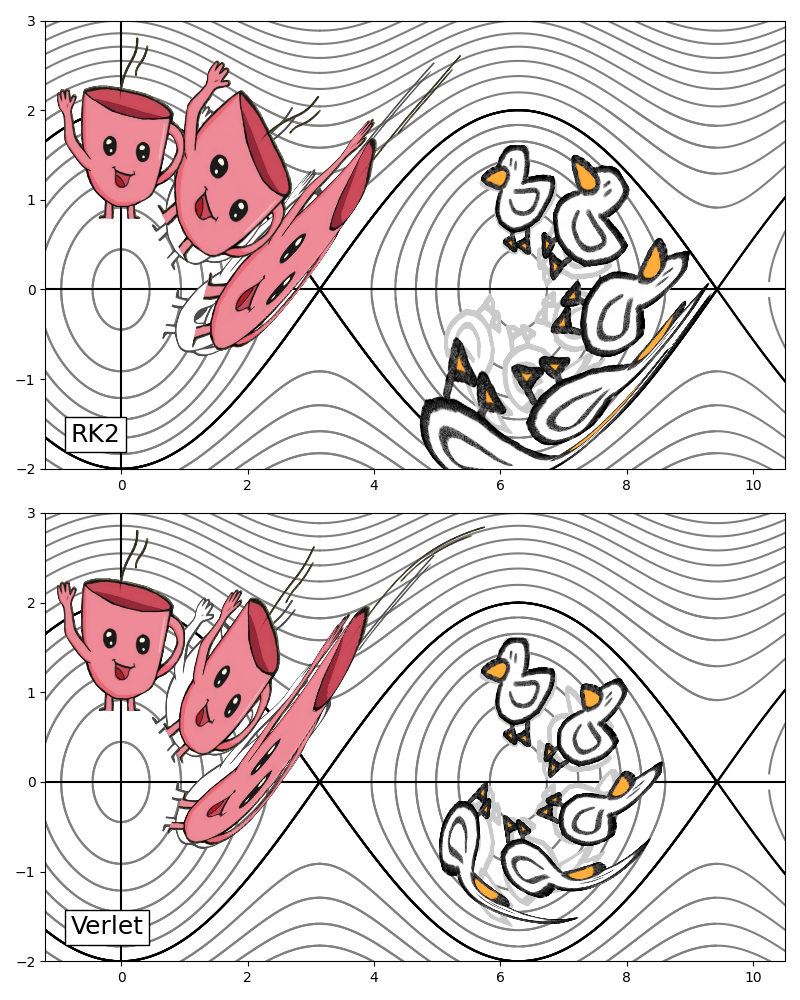
\includegraphics[width=0.47\linewidth]{python/pendulo/ordem2.png}
    \caption{Métodos RK22 (Exp.) e Velocity-Verlet aplicados no pêndulo com $dt = \pi/3$.}
\end{figure}

\end{frame}

%------------------------------------------------

\begin{frame}
\justifying
\frametitle{Métodos de Ruth (8/13)}

Métodos de ordem mais alta podem ser obtidos através da fórmula de Baker-Campbell-Hausdorff (BCH).

\begin{exampleblock}{Ruth de 3ª Ordem \cite{ruth3}}
    \begin{align*}
        c_1 = 1,    & \quad & c_2 = -2/3, & \quad & c_3 = 2/3, \\
        d_1 = -1/24 & \quad & d_2 = 3/4,  & \quad & d_3 = 7/24.
    \end{align*}
\end{exampleblock}

\begin{exampleblock}{Ruth de 4ª Ordem \cite{ruth4}}
    \begin{align*}
        c_1 = c_4 = \dfrac{1}{2(2-2^{1/3})}, & \quad & c_2 = c_3 = \dfrac{1-2^{1/3}}{2(2-2^{1/3})}, \\
        d_1 = d_3 = \dfrac{1}{2-2^{1/3}}, & \quad & d_2 = - \dfrac{2^{1/3}}{2-2^{1/3}}, \quad d_4 = 0.
    \end{align*}
\end{exampleblock}

\end{frame}

%------------------------------------------------

\begin{frame}
\justifying
\frametitle{Métodos de alta ordem via composição de métodos simétricos (9/13)}

Se $\vet \Phi_{h}$ é o método de Verlet, podemos obter um método de ordem (par) mais alta que é simplético, simétrico e reversível. Estes são os Störmer-Verlet Compostos (SVC):
$$
\vet \Psi_h = \vet \Phi_{\gamma_s h} \circ \hdots \circ \vet \Phi_{\gamma_2 h} \circ \vet \Phi_{\gamma_1 h}.
$$
\pause
\begin{alertblock}{}
    \textbf{Desvantagem:} Precisamos de muitos estágios para aumentar a ordem!
\end{alertblock}
\pause
\begin{exampleblock}{Métodos de ordem 8 e 10 \cite{hairer}}
\begin{itemize}
    \item Métodos SVC de 8ª ordem precisam de 15 estágios;

    \item Métodos SVC de 10ª ordem precisam de 31 estágios.
\end{itemize}
\end{exampleblock}

\end{frame}

%------------------------------------------------

\begin{frame}
\justifying
\frametitle{Há métodos de Runge-Kutta Simpléticos? (10/13)}

\begin{block}{Runge-Kuttas Simpléticos \cite[p.192]{hairer}}
    \textbf{Teorema:} Se os coeficientes de um método de Runge-Kutta de $R$ estágios são tais que
    $$
    b_i a_{ij} + b_j a_{ji} - b_i b_j = 0, \quad i, j = 1, ..., R,
    $$
    então o método é simplético.
\end{block}
\begin{alertblock}{}
    \textbf{Desvantagem:} Todo método de Runge-Kutta simplético é implícito!
\end{alertblock}

\end{frame}

%------------------------------------------------

\begin{frame}
\justifying
\frametitle{Métodos de Runge-Kutta-Nyström (RKN) (11/13)}

Se $T(\vet p) = \frac{1}{2} \vet p^T \bm M^{-1} \vet p$ e $-\nabla_{\vet q_a} V(\vet q) = \vet F_a(\vet q)$, temos um método RKN:
\begin{align*}
    \vet y_i & = \vet q_k + c_i h \dfrac{\vet p_k}{m} + h^2 \sum_{j=1}^{s} a_{ij} \dfrac{\vet F(\vet y_i)}{m}, \quad i = 1, 2, ..., s, \\
    \vet q_{k+1} &= \vet q_k + h \dfrac{\vet p_k}{m} + h^2 \sum_{i=1}^{s} b_i \dfrac{\vet F(\vet y_i)}{m}, \\
    \vet p_{k+1} &= \vet p_k + h \sum_{i=1}^{s} B_i \vet F(\vet y_i),
\end{align*}
para constantes $\bm A, \vet b, \vet c$ e $B_1, ..., B_s$.

\begin{exampleblock}{\cite{okunbor}}
\begin{itemize}
    \item RKN551: Runge-Kutta-Nyström de 5ª ordem e 5 estágios.
    \item RKN671: Runge-Kutta-Nyström de 6ª ordem e 7 estágios.
\end{itemize}
\end{exampleblock}

\end{frame}

%------------------------------------------------

\begin{frame}
\justifying
\frametitle{Métodos simpléticos implementados (12/13)}

\begin{center}
    \begin{tabular}{|c|c|c|c|}
    \hline
    \textbf{Método} & \textbf{Ordem} & \textbf{Estágios} & \textbf{Autoria}
    \\ \hline
    Euler Simplético & 1 & 1 & de Vogelaere, 1956
    \\ \hline
    Velocity-Verlet & 2 & 2 & de Vogelaere, 1956
    \\ \hline
    Ruth3 & 3 & 3 & Ruth, 1983
    \\ \hline
    Ruth4 & 4 & 4 & Forest \& Ruth, 1990
    \\ \hline
    ecp4s5 & 4 & 5 & McLachlan, 1995
    \\ \hline
    ecp4s6 & 4 & 6 & Blanes \& Moan, 2002
    \\ \hline
    RKN551 & 5 & 5 & Okunbor \& Skeel, 1994
    \\ \hline
    RKN671 & 6 & 7 & Okunbor \& Skeel, 1994
    \\ \hline
    svcp6s9 & 6 & 9 & Kahan \& Li, 1997
    \\ \hline
    svcp8s15 & 8 & 15 & Suzuki \& Umeno, 1993
    \\ \hline
    svcp10s35 & 10 & 35 & Sofroniou \& Spaletta (2004)
    \\ \hline
    \end{tabular}
\end{center}

\end{frame}

%------------------------------------------------

% \begin{frame}
% \justifying
% \frametitle{Comparação dos métodos simpléticos implementados (10/?)}

% \begin{figure}
%     \centering
%     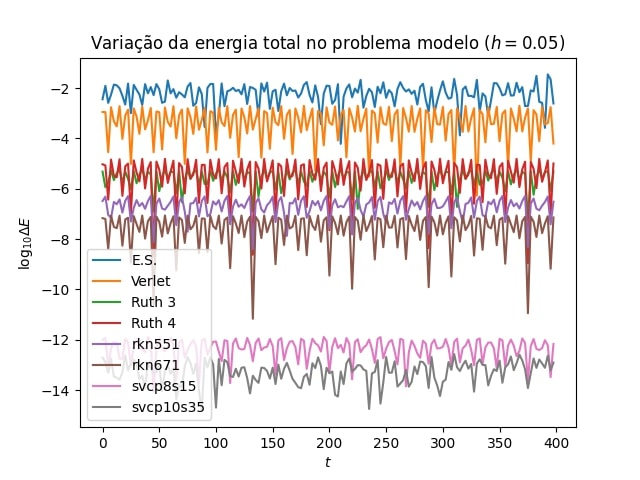
\includegraphics[width=0.8\linewidth]{img/var_energia_simpleticos.jpg}
%     \caption{Variação da energia total para os métodos simpléticos apresentados. A lemniscata foi integrada no intervalo $[0, 400]$ com tamanho de passo $h = 0.05$.}
% \end{figure}

% \end{frame}

% \begin{frame}
% \justifying
% \frametitle{Comparação dos métodos simpléticos implementados (10/?)}

% \begin{figure}
%     \centering
%     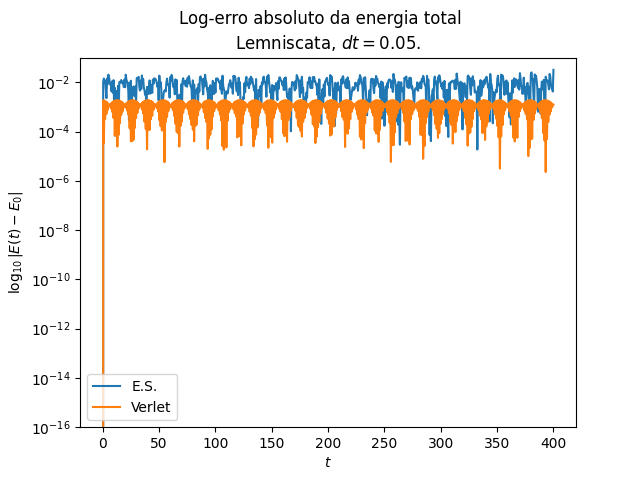
\includegraphics[width=0.8\linewidth]{energia/simpleticos/lemniscata_metodos_simpleticos_energia_1.png}
%     \caption{Variação da energia total para os métodos simpléticos apresentados. A lemniscata foi integrada no intervalo $[0, 400]$ com tamanho de passo $h = 0.05$.}
% \end{figure}

% \end{frame}

% \begin{frame}
% \justifying
% \frametitle{Comparação dos métodos simpléticos implementados (10/?)}

% \begin{figure}
%     \centering
%     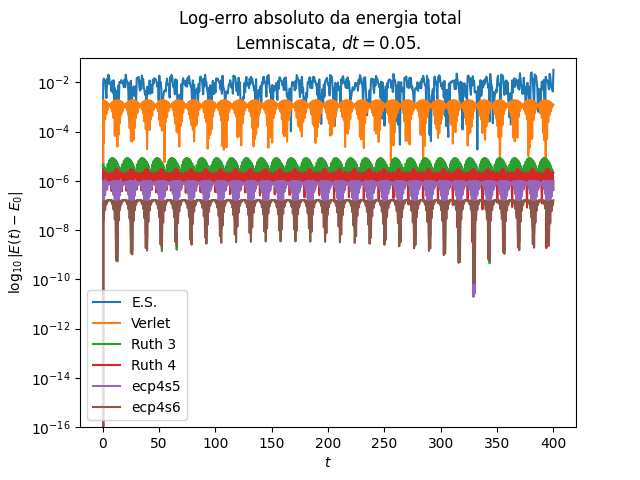
\includegraphics[width=0.8\linewidth]{energia/simpleticos/lemniscata_metodos_simpleticos_energia_2.png}
%     \caption{Variação da energia total para os métodos simpléticos apresentados. A lemniscata foi integrada no intervalo $[0, 400]$ com tamanho de passo $h = 0.05$.}
% \end{figure}

% \end{frame}

% \begin{frame}
% \justifying
% \frametitle{Comparação dos métodos simpléticos implementados (10/?)}

% \begin{figure}
%     \centering
%     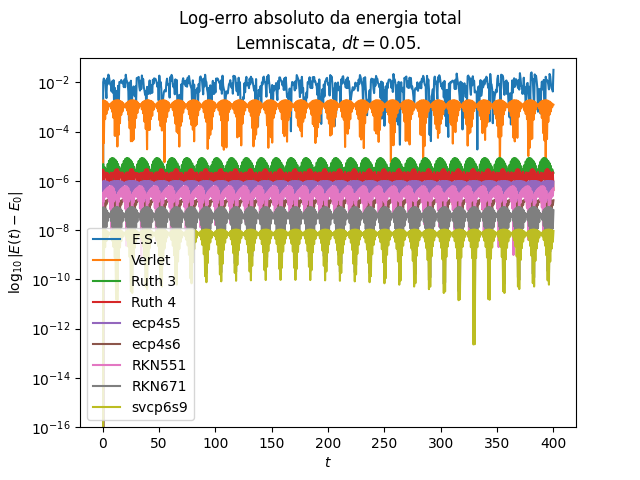
\includegraphics[width=0.8\linewidth]{energia/simpleticos/lemniscata_metodos_simpleticos_energia_3.png}
%     \caption{Variação da energia total para os métodos simpléticos apresentados. A lemniscata foi integrada no intervalo $[0, 400]$ com tamanho de passo $h = 0.05$.}
% \end{figure}

% \end{frame}

\begin{frame}
\justifying
\frametitle{Comparação dos métodos simpléticos implementados (13/13)}

\begin{figure}
    \centering
    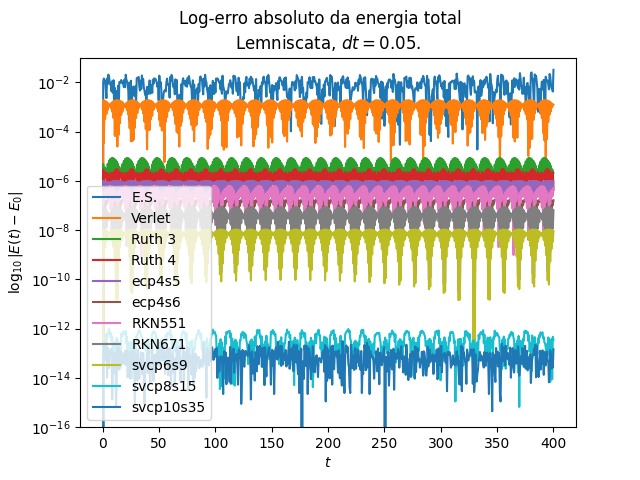
\includegraphics[width=0.8\linewidth]{energia/simpleticos/lemniscata_metodos_simpleticos_energia_4.png}
    \caption{Variação da energia total para os métodos simpléticos apresentados. A lemniscata foi integrada no intervalo $[0, 400]$ com tamanho de passo $h = 0.05$.}
\end{figure}

\end{frame}

%------------------------------------------------

\begin{frame}
\justifying
\frametitle{Corretor numérico \cite{nacozy} (1/3)}

Outra forma de melhorar os resultados é aplicar correções sobre as aproximações.
\pause
\\~\\
Considerando um PVI conservativo e $\vet \Psi = (\psi_1, ..., \psi_k)$ suas $k$ integrais primeiras, se $\vet z^*$ é uma aproximação de $\vet z = \vet z(t^*)$, temos por linearização
\begin{equation*}
    \vet z = \vet z^* + D\vet \Psi(\vet x^*)^T \vet \alpha,
\end{equation*}
onde $\vet \alpha$ resolve
\begin{equation*}
    D\vet \Psi(\vet z^*) D\vet \Psi(\vet z^*)^T \vet \alpha = \vet \Psi(\vet z_0) - \vet \Psi(\vet z^*).
\end{equation*}
\begin{figure}
    \centering
    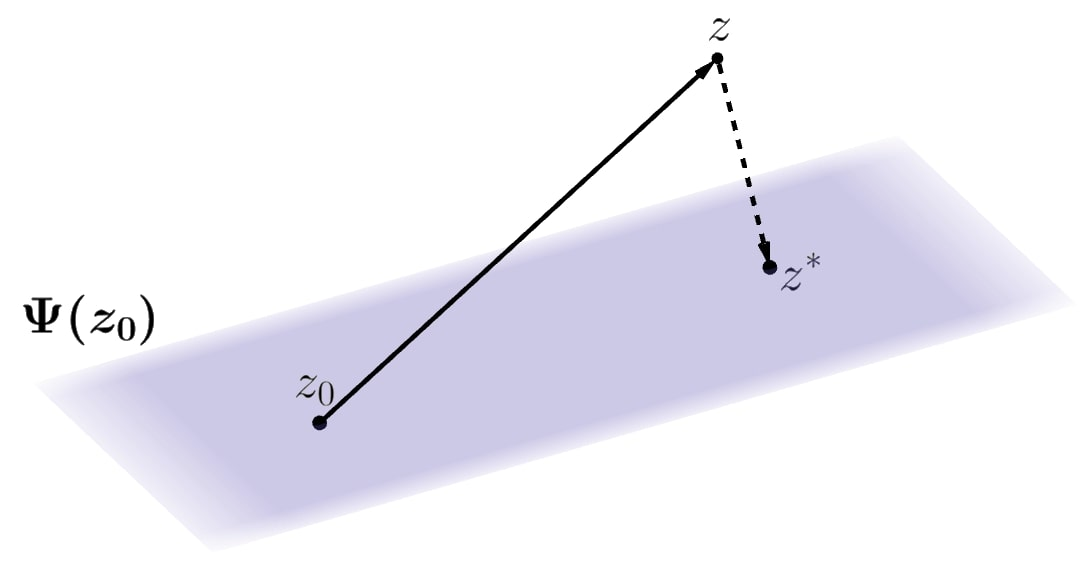
\includegraphics[width=0.5\linewidth]{img/corretor_visualizacao.jpg}
    \caption{Visualização do corretor}
    \label{fig:enter-label}
\end{figure}

\end{frame}

%------------------------------------------------

\begin{frame}
\justifying
\frametitle{Euler Explícito vs Euler Simplético vs Corrigidos (2/3)}

\begin{figure}
    \centering
    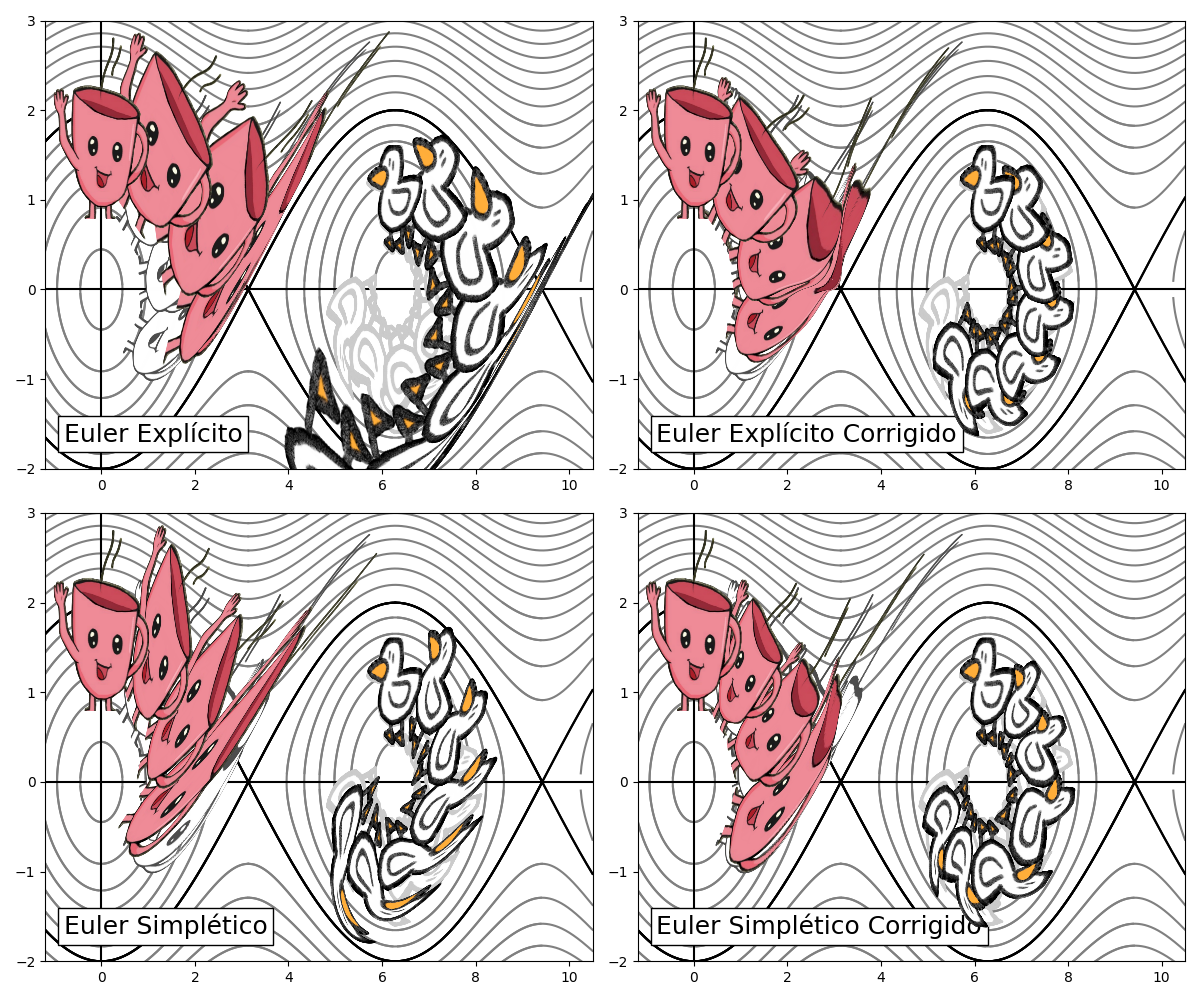
\includegraphics[width=0.57\linewidth]{python/pendulo/corretor.png}
    \caption{Euler Explícito e Euler Simplético originais e corrigidos para o pêndulo com $dt = \pi/3$.}
\end{figure}

\end{frame}

%------------------------------------------------

\begin{frame}
\justifying
\frametitle{Corretor numérico (3/3)}

Vamos testar com o método de Euler explícito na lemniscata:

% \begin{figure}
%     \centering
%     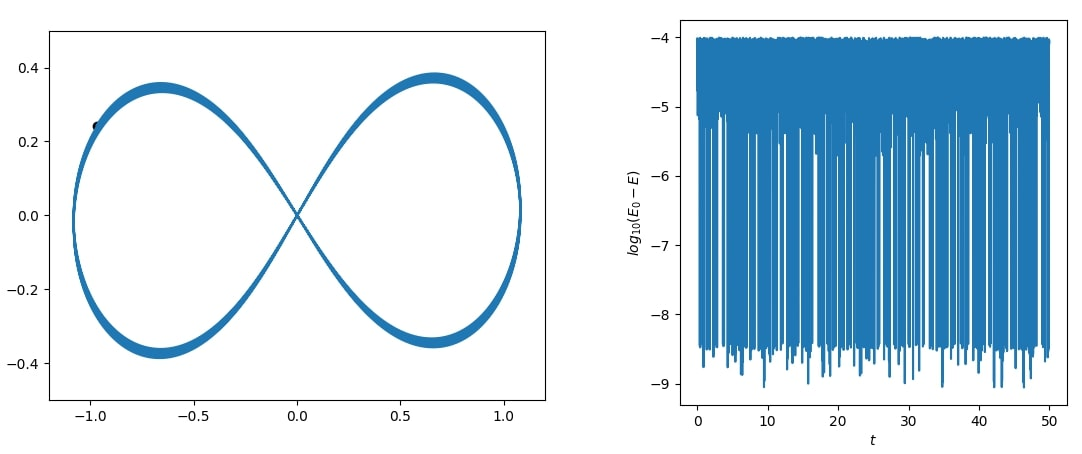
\includegraphics[width=\linewidth]{img/euler_exp_corr.jpg}
%     \caption{Euler explícito com correção ($h=10^{-3}, \epsilon_c=10^{-4}$)}
%     \label{fig:enter-label}
% \end{figure}

\begin{columns}
    \column{.50\textwidth}\justifying
        \begin{figure}
            \centering
            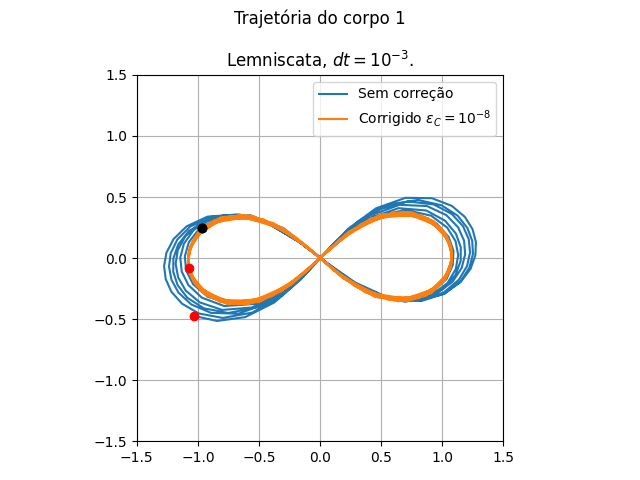
\includegraphics[width=\linewidth]{img/corretor/euler_corrigido_trajetorias.png}
            \caption{Lemniscata}
        \end{figure}

    \column{.50\textwidth}\justifying
        \begin{figure}
            \centering
            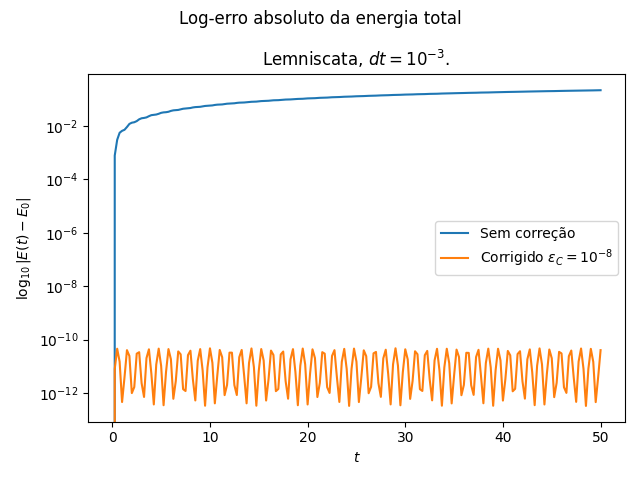
\includegraphics[width=\linewidth]{img/corretor/euler_corrigido.png}
            \caption{Erro na energia}
        \end{figure}
\end{columns}

\end{frame}

%------------------------------------------------

\begin{frame}
\justifying
\frametitle{Métodos multipasso (1/3)}

\begin{block}{Métodos multipasso lineares}
\begin{itemize}
    \item Em vez de fazer médias de derivadas, podemos usar valores de passos anteriores para obter aproximações.

    \begin{equation*}
        y_{k+n} = - \sum_{j=0}^{n-1} \alpha_j y_{k+j} + h \sum_{j=0}^{n} \beta_{k+j} f(t_{k+j}, y_{k+j}).
    \end{equation*}

    \item Enquanto Runge-Kuttas fazem muitos cálculos e descartam a maioria, os métodos multipasso reaproveitam o que já foi calculado.
\end{itemize}
\end{block}

\begin{exampleblock}{Adams-Bashforth de 2 passos e ordem 2}
    \begin{equation*}
        y_{k+2} = y_{k+1} + \dfrac{h}{2} \left(3 f(t_{k+1}, y_{k+1})-f(t_k, y_k)\right)
    \end{equation*}
\end{exampleblock}

\end{frame}

%------------------------------------------------

\begin{frame}
\justifying
\frametitle{Métodos multipasso (2/3)}

\begin{exampleblock}{Vantagens}
\begin{itemize}
    \item Em métodos explícitos, só é preciso calcular $f$ uma vez.
    \item Fáceis de se implementar e analisar.
    \item Existe um método de passo único que produz exatamente os mesmos resultados. \cite[pp.573-576]{hairer}
    \item Métodos simétricos preservam aproximadamente uma hamiltoniana perturbada.
\end{itemize}
\end{exampleblock}
\pause
\begin{alertblock}{Desvantagens}
\begin{itemize}
    \item Só funcionam sob trajetórias contínuas.
    \item \textbf{(Tang, 1993)} O método de passo único adjacente não pode ser simplético.
    \item Os modos parasitas podem acumular erros expressivos ao longo do tempo.
\end{itemize}
\end{alertblock}

\end{frame}

%------------------------------------------------

\begin{frame}
\justifying
\frametitle{Métodos multipasso (3/3)}

\begin{figure}
    \centering
    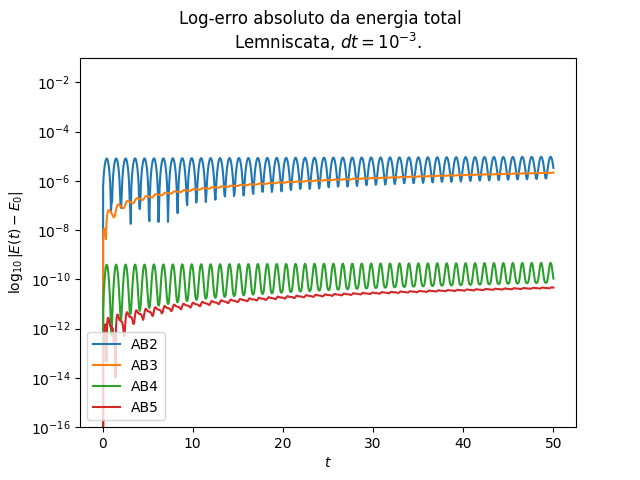
\includegraphics[width=\linewidth]{energia/lemniscata_metodos_multipasso.png}
    \caption{Métodos multipasso implementados.}
    \label{fig:energia_multipassos}
\end{figure}

\end{frame}

%------------------------------------------------

\begin{frame}
\justifying
\frametitle{Comparação de tempo entre os métodos}

\begin{figure}
    \centering
    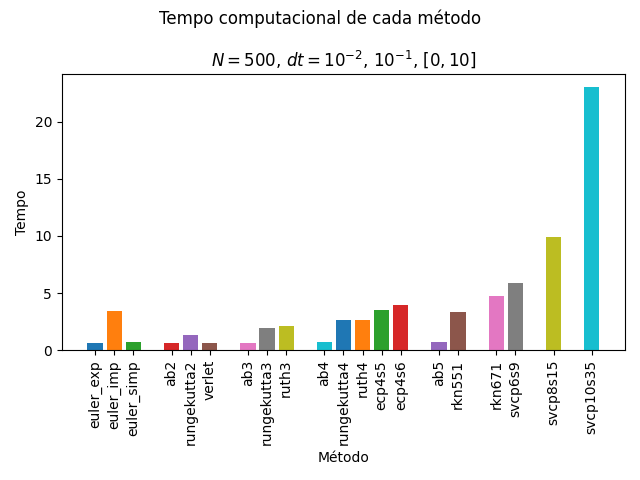
\includegraphics[width=\linewidth]{energia/tempo_geral.png}
    \caption{Comparação de tempo entre todos os métodos implementados.}
    \label{fig:tempo_geral}
\end{figure}

\end{frame}

%------------------------------------------------